\subsection*{I. Pr{\'e}ambule}
\begin{enumerate}
 \item Le point important est la pr{\'e}sence du $\forall \varepsilon$ dans la d{\'e}finition d'un point de franchissemement.\newline
 Soit $t_{0}$ un point de franchissement vers le haut et $\varepsilon_{0}$ tel que
 \begin{displaymath}
  f < u  \text{ dans } ]t_{0}-\varepsilon _{0}, t_{0}[, \;
  f>u \text{ dans } ]t_{0}, t_{0}+\varepsilon _{0}[.
 \end{displaymath}
 Pour tout $\varepsilon >0$, $] t_{0}-\varepsilon ,t_{0}[ \cap ]t_{0}-\varepsilon ,t_{0}[ =] t_{0}-\min (\varepsilon ,\varepsilon_{0}),t_{0}[ \neq \emptyset$ et si $t_{1}$ est dans cet intervalle $f(t_{1})<u$.
 De m{\^e}me, $] t_{0},t_{0}+\varepsilon [\cap ] t_{0},t_{0}+\varepsilon [ =] t_{0},t_{0}+\min (\varepsilon,\varepsilon _{0})[ \neq \emptyset $ et si $t_{2}$ est dans cet intervalle $f(t_{2})>u$.

  \item  Soit $t_{0}$ un point de franchissement. D'apr{\`e}s la d{\'e}finition d'un tel point, pour tout entier $n>0$, il existe $t_{n}^{+}$ et $t_{n}^{-}$
  dans $]t_{0}-\frac{1}{n},t_{0}+\frac{1}{n}[ $ tels que $f(t_{n}^{-})<u$ et $f(t_{n}^{+})>u$.
  Le th{\'e}or{\`e}me des valeurs interm{\'e}daires prouve l'existence d'un $x_{n}$ entre $t_{n}^{-}$ et $t_{n}^{+}$ donc dans
  $]t_{0}-\frac{1}{n},t_{0}+\frac{1}{n}[ $ et tel que $f(x_{n})=u$.
  D'apr{\`e}s le th{\'e}or{\`e}me d'encadrement $(x_{n})_{n\in \mathbf{N}}$ converge vers $t_{0}$ et $f(t_{0})=u$ par continuit{\'e}.

  \item  Dans les cas a., b., c. le point $\frac{1}{2}$ est un point de franchissement de $0$ vers le haut. Dans les cas d. et e. il ne s'agit pas d'un point de franchissement.

  \item  Je vais montrer la proposition contrapos{\'e}e. Supposons que $t_{0}$ soit un point de franchissement et qu'il existe un $\alpha >0$ tel que dans
  $] t_{0}-\alpha ,t_{0}+\alpha [ $ $f$ prenne un nombre fini de fois la valeur $u$ (elle la prend au moins en $t_{0})$ par exemple en $\{ t_{0},t_{1},\cdots ,t_{s}\}$.
  Soit $\beta $ la distance minimale entre $t_{0}$ et un autre de ces points, alors $f-u$ garde un signe constant dans $] t_{0}-\beta ,t_{0}[ $ et dans $]t_{0},t_{0}+\beta [ $.
  Les deux signes sont diff{\'e}rents car $t_{0}$ est un point de franchissement, on se trouve alors obligatoirement dans le cas d'un franchissement vers le haut ou vers le bas.\newline
  Par contraposition, si $t_{0}$ est un point de franchissement qui n'est ni vers le haut ni vers le bas, la fonction $f$ prend une infinit{\'e} de fois la valeur $u$ dans un intervalle ouvert quelconque autour de $t_{0}$. Un exemple de fonction de ce type est
\begin{displaymath}
  f(x) =
  \left\lbrace
    \begin{align*}
      | x-\frac{1}{2}| \sin \frac{1}{x-\frac{1}{2}} & \text{ si } & x\neq \frac{1}{2} \\
      0                                             & \text{ si } & x=\frac{1}{2}
    \end{align*}
  \right.
\end{displaymath}
Cette fonction est continue dans $[ 0,1] $ car $| f(x)| \leq | x-\frac{1}{2}| $ assure la continuit{\'e} en $\frac{1}{2}.$ Ce point est un point de franchissement de $0$ qui
n'est ni vers le haut ni vers le bas, son graphe est :
\begin{figure}
   \centering
   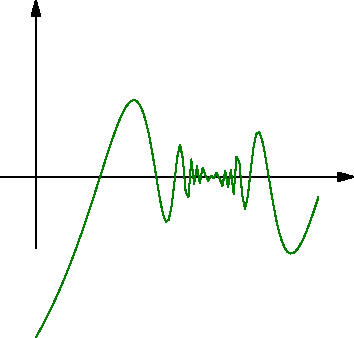
\includegraphics{Cfranch_1.pdf}
   \caption{I.4. Point de franchissement ni vers le haut ni vers le bas.}
\end{figure}

  \item  Soit $t_{0}$ un point qui n'est pas de franchissement et tel que $f(t_{0})=u$. Il existe alors un $\alpha >0$ tel que $f-u$ garde un
signe constant dans $] t_{0}-\alpha ,t_{0}+\alpha [ $. Si $f-u$ est positif $t_{0}$ est un minimum local, si $f-u$ est n{\'e}gatif c'est un maximum local.

  \item  Supposons $f(t_{1})>u$ et $f(t_{2})<u$ avec $t_{1}<t_{2}$ pour fixer les id{\'e}es (l'autre cas est analogue). Consid{\'e}rons
$A=\{ t\in [ t_{1},t_{2}] \text{ tels que }f(t)>u\} $. Cet ensemble est non vide ( $t_{1}\in A$), major{\'e} par $t_{2}$ il admet une borne sup{\'e}rieure que je note $t_{0}$. Montrons que
$t_{0}$ est un point de franchissement.

  \begin{itemize}
    \item  Il existe une suite d'{\'e}l{\'e}ments de $A$ qui converge vers $t_{0}.$ On en d{\'e}duit, par passage {\`a} la limite dans une
in{\'e}galit{\'e} et par continuit{\'e} que $f(t_{0})\geq u$. Ceci assure $t_{0}<t_{2}$.

    \item  $A\cap ] t_{0},t_{2}] $ est vide car $t_{0}=\sup A$ donc $\forall t\in ] t_{0},t_{2}] $, $f(t)\leq u$ en fait on a m{\^e}me
    $f(t)<u$ sinon $f$ serait constante sur $] t_{0},t] $. Ceci prouve que pour tout $\varepsilon >0$, il existe un
    $\theta _{1}\in ]t_{0},t_{0}+\varepsilon [ $ tel que $f(\theta _{1})<u$.

    \item  Pour tout $\varepsilon >0$, $t_{0}-\varepsilon $ n'est pas un majorant de $A,$ il existe donc un $\theta _{2}\in ]t_{0}-\varepsilon ,t_{0}[ \cap A$ donc tel que
    $f(\theta _{2})>u$.
  \end{itemize}
\end{enumerate}

\subsection*{II. Polygonation}
\begin{enumerate}
 \item Une fonction affine est continue, la restriction de $f_{n}$ sur chaque segment est donc continue. Ceci montre que $f_{n}$ est
continue sur chaque intrevalle ouvert $]\frac{k}{2^{n}},\frac{k+1}{2^{n}}[ $. De plus la limite {\`a} droite en $\frac{k}{2^{n}}$ est {\'e}gale {\`a} sa limite {\`a}
droite et {\`a} $f(\frac{k}{2^{n}})$ ce qui d{\'e}montre la continuit{\'e} aux points de la subdivision. Elle n'est jamais constante de valeur $u$ car $f$ ne prend pas la valeur $u$ aux points de la forme $\frac{k}{2^{n}}$.

  \item Le segment $[ 0,1] $ se d{\'e}compose en un nombre fini d'intervalles sur lesquels $f_{n}$ est strictement monotone ou
constante d'une valeur $\neq u$. Sur chacun de ces intervalles, $f_{n}$ prend au plus une fois la valeur $u$. Chacun de ces points est de franchissement, $F_{u}^{n}$ est donc le nombre d'intervalles o{\`u} $f_{n}$ prend la valeur $u $.\newline
Examinons un tel intervalle : aux extr{\'e}mit{\'e}s, les valeurs de $f_{n}$ et de $f$ sont {\'e}gales et de part et d'autre de $u$.
D'apr{\`e}s la question I.6., $f$ admet au moins un point de franchissement sur un tel intervalle donc $F_{u}^{n}\leq F_{u}$.

  \item La $n+1$ i{\`e}me subdivision s'obtient {\`a} partir de la $n$ i{\`e}me en divisant chaque intervalle en deux.
Consid{\'e}rons un intervalle de la subdivision d'ordre $n$ sur lequel $f_{n}$ prend la valeur $u$. Les valeurs de $f$ aux extr{\'e}mit{\'e}s sont de part et d'autre de
$u$ donc il en est de m{\^e}me entre une extr{\'e}mit{\'e} et la valeur de $f_{n} $ au milieu. Ceci montre que $f_{n+1}-u$ s'annule exactement une fois sur un intervalle o{\`u} $f_{n}-u$ s'annule.
Comme $f_{n+1}-u$ peut s'annuler ailleurs, $F_{u}^{n}\leq F_{u}^{n+1}$.

  \item
  \begin{enumerate}
    \item Num{\'e}rotons par ordre croissant les points de franchissement soit $t_{1},\cdots ,t_{F_{u}}$.
Posons $\alpha =\min \{t_{1},t_{2-}t_{1},\cdots ,t_{F_{u}}-t_{F_{u}-1},1-t_{F_{u}}\} $ et
$I_{k}=] t_{k}-\alpha ,t_{k}+\alpha [ $.
Par d{\'e}finition de $\alpha $, $I_{k}$ ne contient pas d'autre point de franchissement que $t_{k}$.

    \item Soit $i\in \{ 1,\cdots ,F_{u}\} $ $I_{i}$ l'intervalle d{\'e}fini dans la question pr{\'e}c{\'e}dente.
Comme $t_{i}$ est un point de franchissement, il existe $\theta _{1}$ et $\theta_{2}$ dans $I_{i}$ tels que $f(\theta _{1})>u$ et $f(\theta_{2})<u$.
Comme $f$ est continue en $\theta _{1}$, il existe $J_{i}$ assez petit pour {\^e}tre inclus dans $I_{i} $ et pour que $f-u$ reste strictement positive dans $J_{i}$.
De m{\^e}me, l'existence de $K_{i}$ est assur{\'e}e par la continuit{\'e} de $f$ en $\theta _{2}$.

    \item Lorsque $2^{-n}$ est plus petit que la plus petite longueur des intervalles $J_{i}$ et $K_{i}$ de la question pr{\'e}c{\'e}dente, chaque point de franchissement se trouve dans
un seul des intervalles de la subdivision associ{\'e}e {\`a} $f_{n}$, chacun de ces intervalles contient
exactement un des points de franchissement donc $F_{u}^{n}=F_{u}$.
La suite $(F_{u}^{n})_{n\in \mathbf{N}}$ est stationnaire de valeur $F_{u}$.
  \end{enumerate}

  \item Donnons nous $K$ (entier arbitraire) points de franchissements $t_{1},t_{2},\cdots ,t_{K}$.\newline
Soit $\delta $ un nombre inf{\'e}rieur {\`a} la plus petite distance entre deux de ces points.
Il existe alors $y_{i}$, $z_{i}$ dans $] t_{i}-\delta ,t_{i}+\delta [ $ tels que $f(y_{i})>u$, $f(z_{i})<u$.
On suppose $y_{i}<z_{i}$ pour fixer les id{\'e}es.
Je me propose de montrer que, pour $n$ assez grand, $f_{n}$ admet un point de franchissement de $u$ entre $y_{i}$ et $z_{i}$.
Ce qui entra\^{i}nera $F_{u}^{n}\geq K$ et donc $(F_{u}^{n})_{n\in \mathbf{N}} \rightarrow +\infty $.\newline
La d{\'e}finition de $\delta $ montre que les $y_{i}$ et $z_{i}$ sont deux {\`a} deux distincts.
Soit $\varepsilon >0$ le plus petit des nombres $f(y_{i})-u$ et $u-f(z_{i})$. A cause de l'\emph{uniforme continuit{\'e}}, il existe un $\alpha >0$ tel que
$| f(x)-f(y)| <\varepsilon $ d{\`e}s que $| x-y| <\alpha $.\newline
Lorsque $\frac{1}{2^{n}}<\alpha $ et que $a$ et $b$ sont deux entiers tels que
\[
\frac{a-1}{2^{n}}\leq y_{i}<\frac{a}{2^{n}}<\cdots
<\frac{b}{2^{n}}\leq z_{i}<\frac{b+1}{2^{n}}.
\]
On a aussi $f(\frac{a}{2^{n}})>u$ et $f(\frac{b}{2^{n}})<u$.
Il existe alors un entier $k$ entre $a$ et $b$ tel que $f(\frac{k}{2^{n}})>u$ et $f(\frac{k+1}{2^{n}})<u$, ce qui prouve que $f_{n}$ admet un point de
franchissement dans $] \frac{k}{2^{n}},\frac{k+1}{2^{n}}[ $.

  \item La fonction $(x-\frac{1}{2})| \sin \frac{1}{(x-\frac{1}{2})}| $ admet en $\frac{1}{2}$ un point de franchissement qui n'est ni vers le haut ni vers
le bas. C'est le seul point de franchissement de $0$, tous les points o{\`u} $f$ prend la valeur 0 sont des points de tangence.\newline
Montrons que $F_{u}$ infini entra\^{i}ne que $f$ admet un point de franchissement de $u$ qui n'est ni vers le haut ni vers le bas.

On raisonne par dichotomie en s'inspirant de la d{\'e}monstration du th{\'e}or{\`e}me de Bolzano-Weirstrass.\newline
%\begin{floatingfigure}{5cm}
%\incluregraphics[height=5cm,width=5cm]{F2franch.pdf} include au lieu de inclure
%\end{floatingfigure}
Coupons $I_{0}=[ 0,1] $ en deux, une des deux moiti{\'e}s doit contenir une infinit{\'e} de points de franchissement, on l'appelle $I_{1}$.
De m{\^e}me une des deux moiti{\'e}s (soit $I_{2}$) de $I_{1}$ contiendra une infinit{\'e} de points de franchissements.
On construit ainsi une suite de segments embo\^{i}t{\'e}s dont les extr{\'e}mit{\'e}s $x_{n}$ et $y_{n}$ forment des suites adjacentes qui convergent vers un
$t_{0}\in [0,1] $.\newline
Soit $\theta _{n}$ un point de franchissement dans $[ x_{n},y_{n}] $ alors $f(\theta _{n})=u$.
Comme $(\theta _{n})_{n\in \mathbf{N}} \rightarrow t_{0}$, $f(t_{0})=u$ par continuit{\'e}.
Ceci prouve aussi que $t_{0}\in ] x_{n},y_{n}[ $ car $x_{n}$ et $y_{n}$ sont de la forme $\frac{k}{2^{n}}$ et que $f$ ne prend pas la valeur $u$ en ces points.\newline
Pour tout $\varepsilon >0$, il existe un $n$ tel que $t_{0}-\varepsilon <x_{n}<t_{0}<y_{n}<t_{0}+\varepsilon $.
Un des deux intervalles $]x_{n},t_{0}[ $ ou $] t_{0},y_{n}[ $ contient une infinit{\'e} de points de franchissements, par exemple $] x_{n},t_{0}[$.
Soit $\theta $ l'un d'entre eux.\newline
Pour $\alpha =\min (t_{0}-\theta ,\theta -x_{n})$, il existe $t_{1}$ et $t_{2}$ dans
$] \theta -\alpha ,\theta +\alpha [ \subset ] x_{n},t_{0}[ \subset ] t_{0}-\varepsilon ,t_{0}+\varepsilon [ $
tel que $f(t_{1})>u$, $f(t_{2})<u$.
Ceci prouve que $t_{0}$ est un point de franchissement et qu'il n'est ni vers le haut ni vers le bas.
\end{enumerate}
